\documentclass[a4paper,14pt]{extreport}
\usepackage[left=1.5cm,right=1.5cm,
    top=1.5cm,bottom=2cm,bindingoffset=0cm]{geometry}
\usepackage{scrextend}
\usepackage[T1,T2A]{fontenc}
\usepackage[utf8]{inputenc}
\linespread{1.5}
\usepackage[english,russian,ukrainian]{babel}
\usepackage{tabularx}
\usepackage{amssymb}
\usepackage{color}
\usepackage{amsmath}
\usepackage{mathrsfs}
\usepackage{listings}
\usepackage{graphicx}
\graphicspath{ {./images/} }
\usepackage{lipsum}
\usepackage{xcolor}
\usepackage{hyperref}
\usepackage{tcolorbox}
\usepackage{tikz}
\usepackage[framemethod=TikZ]{mdframed}
\usepackage{wrapfig,boxedminipage,lipsum}
\mdfdefinestyle{MyFrame}{%
linecolor=blue,outerlinewidth=2pt,roundcorner=20pt,innertopmargin=\baselineskip,innerbottommargin=\baselineskip,innerrightmargin=20pt,innerleftmargin=20pt,backgroundcolor=gray!50!white}
 \usepackage{csvsimple}
 \usepackage{supertabular}
\usepackage{pdflscape}
\usepackage{fancyvrb}
%\usepackage{comment}
\usepackage{array,tabularx}
\usepackage{colortbl}

\usepackage{varwidth}
\tcbuselibrary{skins}
\usepackage{fancybox}
\usepackage{spreadtab}
\usepackage{xstring}
\usepackage{fp}
\usepackage{ulem}


\usepackage{tikz}
\usepackage[framemethod=TikZ]{mdframed}
\usepackage{xcolor}
\usetikzlibrary{calc}
\makeatletter
\newlength{\mylength}
\xdef\CircleFactor{1.1}
\setlength\mylength{\dimexpr\f@size pt}
\newsavebox{\mybox}
\newcommand*\circled[2][draw=blue]{\savebox\mybox{\vbox{\vphantom{WL1/}#1}}\setlength\mylength{\dimexpr\CircleFactor\dimexpr\ht\mybox+\dp\mybox\relax\relax}\tikzset{mystyle/.style={circle,#1,minimum height={\mylength}}}
\tikz[baseline=(char.base)]
\node[mystyle] (char) {#2};}
\makeatother

\definecolor{ggreen}{rgb}{0.4,1,0}
\definecolor{rred}{rgb}{1,0.1,0.1}
\definecolor{amber}{rgb}{1.0, 0.75, 0.0}
\definecolor{babyblue}{rgb}{0.54, 0.81, 0.94}
\definecolor{amethyst}{rgb}{0.6, 0.4, 0.8}
\usepackage{graphicx}
\usepackage{float}
\usepackage{wrapfig}
\usepackage{framed}
%for nice Code{
\lstdefinestyle{customc}{
  belowcaptionskip=1\baselineskip,
  breaklines=true,
  frame=L,
  xleftmargin=\parindent,
  language=C,
  showstringspaces=false,
  basicstyle=\small\ttfamily,
  keywordstyle=\bfseries\color{green!40!black},
  commentstyle=\itshape\color{purple!40!black},
  identifierstyle=\color{blue},
  stringstyle=\color{orange},
}
\lstset{escapechar=@,style=customc}
%}


\begin{document}
\pagecolor{white}

%----------------------------------------1
\newtcbox{\xmybox}[1][red]{on line, arc=7pt,colback=#1!10!white,colframe=#1!50!black, before upper={\rule[-3pt]{0pt}{10pt}},boxrule=1pt, boxsep=0pt,left=6pt,right=6pt,top=2pt,bottom=2pt}

\begin{titlepage}
  \begin{center}
    \large
    Національний технічний університет України \\ "Київський політехнічний інститут імені Ігоря Сікорського"


    Факультет Електроніки

    Кафедра мікроелектроніки
    \vfill

    \textsc{ЗВІТ}\\

    {\Large Про виконання курсової роботи \\
      з дисципліни: «Твердотільна електроніка-3»\\[1cm]

        Варіант №50


    }
  \bigskip
\end{center}
\vfill

\newlength{\ML}
\settowidth{\ML}{«\underline{\hspace{0.4cm}}» \underline{\hspace{2cm}}}
\hfill
\begin{minipage}{1\textwidth}
Виконавець:\\
Студент 3-го курсу \hspace{4cm} $\underset{\text{(підпис)}}{\underline{\hspace{0.2\textwidth}}}$  \hspace{1cm}А.\,С.~Мнацаканов\\
\vspace{1cm}

Перевірив: \hspace{6.1cm} $\underset{\text{(підпис)}}{\underline{\hspace{0.2\textwidth}}}$  \hspace{1cm}Л.\,М.~Королевич\\

\end{minipage}

\vfill

\begin{center}
2021
\end{center}
\end{titlepage}

\newpage
\setcounter{page}{1}


\begin{center}
    \textbf{Завдання}
\end{center}
Розрахувати геометричні розміри транзисторів


\begin{center}
  \textbf{Виконання завдання}
\end{center}

\begin{figure}[h!]
\center{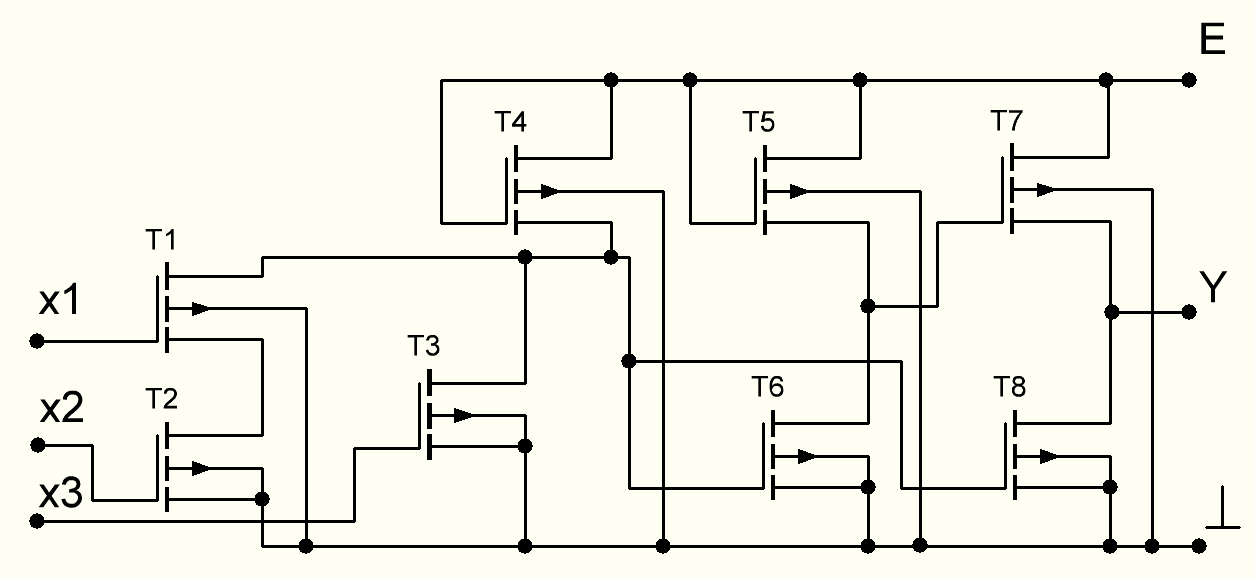
\includegraphics[width=0.8\linewidth]{1.png}}
\caption{Прототип схеми.}
\label{ris1}
\end{figure}

Перш за все запишу всі константи, які знадобляться:\\

\begin{minipage}{0.5\textwidth}
    \begin{flushleft}
  
  $\varepsilon_{0}=8,85 \cdot 10^{-14} \text{ }\dfrac{\text{Ф}}{\text{см}}$\\
  \vspace{0.2cm}
  $\varepsilon_{ox}=3,9$\\
  \vspace{0.2cm}
  $\varepsilon_{S}=11,8$\\
  \vspace{0.2cm}
  $ d_{o x}=100 \text{ } \text{нм}$\\
  \vspace{0.2cm}
  $ N_{B}=8,3 \cdot 10^{14}\text{ } \text{см}^{-3}$\\
  \vspace{0.2cm}
  $ U_{\text{nop.}}^{0}=-5,5 \text{ }\text{B}$\\
  \vspace{0.2cm}
  $ \rho_{s}=100 \text{ }\text{Ом}$\\
  \vspace{0.2 cm}
  $U_{\text{ЗЗ}} = 0 $ В -- напруга на затворі пристрою захисту.\\
  \vspace{0.2 cm}
  $W_{T_1 T_2} = 110 $ мкм\\
  \vspace{0.2 cm}
  $W_{T_3} = 55 $ мкм\\ 


    \end{flushleft}
  \end{minipage}
  \begin{minipage}{0.4\textwidth}
    \begin{flushright}
  
	    $\phi_{F}=0,283 B$\\
	    \vspace{0.2cm}
	    $C_{ox}=3,45 \cdot 10^{-8} \text{ }\dfrac{\text{Ф}}{\text{см}^{2}}$\\
	    \vspace{0.2cm}
	    $U^{0}=-1,1 \text{ }\text{B}$\\
	    \vspace{0.2 cm}
	    $ t_{\text{ викл}} = 760 \text{ нс} $\\
	    \vspace{0.2 cm}
	    $ t_{\text{ вкл}} = 100 \text{ нс} $\\
	    \vspace{0.2 cm}
	    $E_{\text{кр}} = 1,2 $ В/см --  критичне поле, що визначає початок ударної іонізації у зоні збіднення кремнію.\\
	    \vspace{0.2 cm}
		$L_T=L_{T_1,T_2, T_3} = 5 $ мкм\\ 

    \end{flushright}
\end{minipage}



Спочатку знайдемо напругу пробою:
\begin{equation}
U_{\text{проб}} = 3 \cdot d_{ox} \cdot E_{\text{кр}} \cdot U_{\text{ЗЗ}} - |U_{\text{пор зах}} |, 
\end{equation}
де $U_{\text{пор зах}}  = U_{\text{пор}}^0$, тому $U_{\text{проб}} =  30,5 $ В\\

Далі шукаємо робочу частоту:
\begin{equation}
	f = \dfrac{2}{t_{\text{вимк}} + t_{\text{вкл}}} = 2,33 \cdot 10^{6} \text{ Гц}
\end{equation}

Тепер шукаємо струмообмежуючий опір.

$$
R_{6} \leq 0,01 \cdot C_{\text{вх}}^{-1} \cdot f_{\text{роб}}^{-1},
$$
де $C_{\text{вх}}=C_{ox} \cdot W_{T} \cdot L_{T}, W_{T}, L_{T}-$ розміри вхідного транзистора.\\
Тоді маємо, що:
$$
\begin{array}{c}
\left.R_{6}\right|_{T_{1}, T_{2}} \leq \frac{0,01}{C_{ox} \cdot W_{T_{1}, T_{2}} \cdot L_{T} \cdot f_{\text{роб}}}=22,\left.6 \text{ Ом} \Rightarrow R_{6}\right|_{T_{1}, T_{2}}=20 \text{ Ом} \\
\left.R_{6}\right|_{T_{3}} \leq \frac{0,01}{C_{o x} \cdot W_{T_{3}} \cdot L_{T} \cdot f_{\text{ роб}}}=45,\left.2 \text{ Ом} \Rightarrow R_{6}\right|_{T_{1}, T_{2}}=40 \text{ Ом}
\end{array}
$$
Потім шукаємо динамічний опір за формулою:
$$
U_{\text{затв}}=U_{\text{проб}}+\left(U_{\text{вх}}-U_{\text{проб}}\right) \cdot \frac{R_{\partial}}{R_{\partial}+R_{6}}
$$
$$
U_{\text{затв}} \leq \frac{2}{3} \cdot U_{\text {npoб.SіO$_2$}}
$$
максимально допустима напруга на затворі вхідного
транзистора; 
$U_{\text{npoб.SіO$_2$}}=E_{\text {проб }} \cdot d_{\text {оx }}$ - напруга пробою діелектрика; $U_{\text {вх}}=5000 \mathrm{~B}$
напруга, від якої наш пристрій захищає. \\
 $E_{\text{проб}}$ обирається по технології, має бути термічне оксилення
  (так як $\varepsilon_{\text{ox}}$), тому цей парамет береться максимальний, тобто $E_{\text{npoб}} = 10 \cdot 10^{6}\text{ } \dfrac{\text{В}}{\text{см}}$. \\


Тоді: $U_{\text {nроб.SiO }_{2}}=100 \mathrm{~B}, \quad U_{\text {затв }} \leq 66,7 \mathrm{~B} \Rightarrow U_{\text {затв }}=60 \mathrm{~B}$. Виразивши Rд, отримаємо, що:
$$
\left.R_{\partial}\right|_{T_{1}, T_{2}} \approx 119  \text{ Ом},\left.R_{\partial}\right|_{T_{3}} \approx 238 \text{ Ом}
$$
Тепер графічно треба знайти ширину.

$$
W_{3 a x . T_{3}} \approx 119  \text{ мкм}_{ \text{і}} W_{ \text{зах} T_{1}, T_{2}} \approx 238  \text{ мкм}
$$


\begin{figure}[h!]
\center{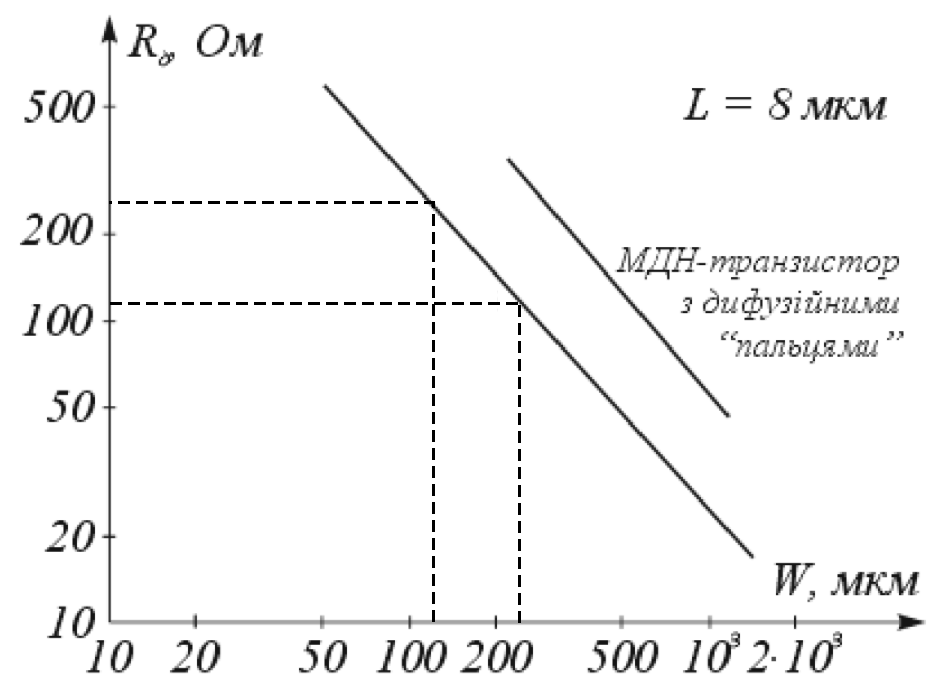
\includegraphics[width=0.8\linewidth]{2.png}}
\caption{Графік для знаходження ширини}
\label{ris2}
\end{figure}

І треба знайти довжину струмообмежуючого опору: $L_{R}=\frac{R_{0} \cdot W_{R}}{\rho_{S}}$, де $\left.W_{R}\right|_{T_{1}, T_{2}, T_{3}}=5 \text{ мкм}$
- ширина дифузійної шини, $\rho_{S}=100 \text{ Ом}-$ питомий опір дифузійної шини.
Тоді
$$
\begin{array}{c}
\left.L_{R}\right|_{T_{1}, T_{2}}=\frac{\left.R_{6}\right|_{T_{1}, T_{2}} \cdot W_{R}}{\rho_{S}}=1000 \text{ мкм} \\
\left.L_{R}\right|_{T_{3}}=\frac{\left.R_{6}\right|_{T_{3}} \cdot W_{R}}{\rho_{S}}=2000 \text{ мкм}
\end{array}
$$
\begin{table}
\caption{ Таблиця розмірів ПЗ для кожного входу}
\begin{tabular}{|c|c|c|c|c|c|c|c|}

\hline & & & & Діод & Діод & Транзистор & Транзистор \\
& $T_{1}$ & $T_{2}$ & $T_{3}$ & $\left(T_{1}, T_{2}\right)$ & $\left(T_{3}\right)$ & $\left(T_{1}, T_{2}\right)$ & $\left(T_{3}\right)$ \\
\hline$W$, \text{ мкм} & 110 & 110 & 55 & 238 & 119 & 5 & 5 \\
\hline L,\text{ мкм} & 5 & 5 & 5 & 5 & 5 & 1000 & 2000 \\
\hline$W / L$ & 22 & 22 & 10,17 & & & & \\
\hline

\end{tabular}

\end{table}












\end{document}
